\documentclass[a4paper]{article}

\setlength{\parskip}{2mm}
\newcommand{\tab}{~ \qquad}
\usepackage{breqn}
\usepackage{ifthen}
\usepackage{amssymb}
\usepackage{multicol}
\usepackage{graphicx}
\usepackage[absolute]{textpos}
\usepackage{amsmath, amscd, amssymb, amsthm, latexsym}
% \usepackage[noload]{qtree}
%\usepackage{xspace,rotating,calligra,dsfont,ifthen}
\usepackage{xspace,rotating,dsfont,ifthen}
\usepackage[spanish,activeacute]{babel}
\usepackage[utf8]{inputenc}
\usepackage{pgfpages}
\usepackage{pgf,pgfarrows,pgfnodes,pgfautomata,pgfheaps,xspace,dsfont}
\usepackage{listings}
\usepackage{multicol}
\usepackage{todonotes}
\usepackage{url}
\usepackage{float}
\usepackage{framed,mdframed}
\usepackage{cancel}

\usepackage[strict]{changepage}


\makeatletter


\newcommand\hfrac[2]{\genfrac{}{}{0pt}{}{#1}{#2}} %\hfrac{}{} es un \frac sin la linea del medio

\newcommand\Wider[2][3em]{% \Wider[3em]{} reduce los m\'argenes
\makebox[\linewidth][c]{%
  \begin{minipage}{\dimexpr\textwidth+#1\relax}
  \raggedright#2
  \end{minipage}%
  }%
}


\@ifclassloaded{beamer}{%
  \newcommand{\tocarEspacios}{%
    \addtolength{\leftskip}{4em}%
    \addtolength{\parindent}{-3em}%
  }%
}
{%
  \usepackage[top=1cm,bottom=2cm,left=1cm,right=1cm]{geometry}%
  \usepackage{color}%
  \newcommand{\tocarEspacios}{%
    \addtolength{\leftskip}{3em}%
    \setlength{\parindent}{0em}%
  }%
}

\newcommand{\encabezadoDeProc}[4]{%
  % Ponemos la palabrita problema en tt
%  \noindent%
  {\normalfont\bfseries\ttfamily proc}%
  % Ponemos el nombre del problema
  \ %
  {\normalfont\ttfamily #2}%
  \
  % Ponemos los parametros
  (#3)%
  \ifthenelse{\equal{#4}{}}{}{%
  \ =\ %
  % Ponemos el nombre del resultado
  {\normalfont\ttfamily #1}%
  % Por ultimo, va el tipo del resultado
  \ : #4}
}

\newcommand{\encabezadoDeTipo}[2]{%
  % Ponemos la palabrita tipo en tt
  {\normalfont\bfseries\ttfamily tipo}%
  % Ponemos el nombre del tipo
  \ %
  {\normalfont\ttfamily #2}%
  \ifthenelse{\equal{#1}{}}{}{$\langle$#1$\rangle$}
}

% Primero definiciones de cosas al estilo title, author, date

\def\materia#1{\gdef\@materia{#1}}
\def\@materia{No especifi\'o la materia}
\def\lamateria{\@materia}

\def\cuatrimestre#1{\gdef\@cuatrimestre{#1}}
\def\@cuatrimestre{No especifi\'o el cuatrimestre}
\def\elcuatrimestre{\@cuatrimestre}

\def\anio#1{\gdef\@anio{#1}}
\def\@anio{No especifi\'o el anio}
\def\elanio{\@anio}

\def\fecha#1{\gdef\@fecha{#1}}
\def\@fecha{\today}
\def\lafecha{\@fecha}

\def\nombre#1{\gdef\@nombre{#1}}
\def\@nombre{No especific'o el nombre}
\def\elnombre{\@nombre}

\def\practicas#1{\gdef\@practica{#1}}
\def\@practica{No especifi\'o el n\'umero de pr\'actica}
\def\lapractica{\@practica}


% Esta macro convierte el numero de cuatrimestre a palabras
\newcommand{\cuatrimestreLindo}{
  \ifthenelse{\equal{\elcuatrimestre}{1}}
  {Primer cuatrimestre}
  {\ifthenelse{\equal{\elcuatrimestre}{2}}
  {Segundo cuatrimestre}
  {Verano}}
}


\newcommand{\depto}{{UBA -- Facultad de Ciencias Exactas y Naturales --
      Departamento de Computaci\'on}}

\newcommand{\titulopractica}{
  \centerline{\depto}
  \vspace{1ex}
  \centerline{{\Large\lamateria}}
  \vspace{0.5ex}
  \centerline{\cuatrimestreLindo de \elanio}
  \vspace{2ex}
  \centerline{{\huge Pr\'actica \lapractica -- \elnombre}}
  \vspace{5ex}
  \arreglarincisos
  \newcounter{ejercicio}
  \newenvironment{ejercicio}{\stepcounter{ejercicio}\textbf{Ejercicio
      \theejercicio}%
    \renewcommand\@currentlabel{\theejercicio}%
  }{\vspace{0.2cm}}
}


\newcommand{\titulotp}{
  \centerline{\depto}
  \vspace{1ex}
  \centerline{{\Large\lamateria}}
  \vspace{0.5ex}
  \centerline{\cuatrimestreLindo de \elanio}
  \vspace{0.5ex}
  \centerline{\lafecha}
  \vspace{2ex}
  \centerline{{\huge\elnombre}}
  \vspace{5ex}
}


%practicas
\newcommand{\practica}[2]{%
    \title{Pr\'actica #1 \\ #2}
    \author{Algoritmos y Estructuras de Datos I}
    \date{Primer Cuatrimestre 2022}

    \maketitlepractica{#1}{#2}
}

\newcommand \maketitlepractica[2] {%
\begin{center}
\begin{tabular}{r cr}
 \begin{tabular}{c}
{\large\bf\textsf{\ Algoritmos y Estructuras de Datos I\ }}\\
Primer Cuatrimestre 2022\\
\title{\normalsize Gu\'ia Pr\'actica #1 \\ \textbf{#2}}\\
\@title
\end{tabular} &
\begin{tabular}{@{} p{1.6cm} @{}}
\includegraphics[width=1.6cm]{logodpt.jpg}
\end{tabular} &
\begin{tabular}{l @{}}
 \emph{Departamento de Computaci\'on} \\
 \emph{Facultad de Ciencias Exactas y Naturales} \\
 \emph{Universidad de Buenos Aires} \\
\end{tabular}
\end{tabular}
\end{center}

\bigskip
}


% Símbolos varios

\newcommand{\nat}{\ensuremath{\mathds{N}}}
\newcommand{\ent}{\ensuremath{\mathds{Z}}}
\newcommand{\float}{\ensuremath{\mathds{R}}}
\newcommand{\bool}{\ensuremath{\mathsf{Bool}}}
\newcommand{\True}{\ensuremath{\mathrm{true}}}
\newcommand{\False}{\ensuremath{\mathrm{false}}}
\newcommand{\Then}{\ensuremath{\rightarrow}}
\newcommand{\Iff}{\ensuremath{\leftrightarrow}}
\newcommand{\implica}{\ensuremath{\longrightarrow}}
\newcommand{\IfThenElse}[3]{\ensuremath{\mathsf{if}\ #1\ \mathsf{then}\ #2\ \mathsf{else}\ #3\ \mathsf{fi}}}
\newcommand{\In}{\textsf{in }}
\newcommand{\Out}{\textsf{out }}
\newcommand{\Inout}{\textsf{inout }}
\newcommand{\yLuego}{\hspace{6pt} \land _L \hspace{6pt}}
\newcommand{\oLuego}{\hspace{6pt} \lor _L \hspace{6pt}}
\newcommand{\implicaLuego}{\implica _L }
\newcommand{\cuantificador}[5]{%
	\ensuremath{(#2 #3: #4)\ (%
		\ifthenelse{\equal{#1}{unalinea}}{
			#5
		}{
			$ % exiting math mode
			\begin{adjustwidth}{+2em}{}
			$#5$%
			\end{adjustwidth}%
			$ % entering math mode
		}
	)}
}

\newcommand{\existe}[4][]{%
	\cuantificador{#1}{\exists}{#2}{#3}{#4}
}
\newcommand{\paraTodo}[4][]{%
	\cuantificador{#1}{\forall}{#2}{#3}{#4}
}

% Símbolo para marcar los ejercicios importantes (estrellita)
\newcommand\importante{\raisebox{0.5pt}{\ensuremath{\bigstar}}}


\newcommand{\rango}[2]{[#1\twodots#2]}
\newcommand{\comp}[2]{[\,#1\,|\,#2\,]}

\newcommand{\rangoac}[2]{(#1\twodots#2]}
\newcommand{\rangoca}[2]{[#1\twodots#2)}
\newcommand{\rangoaa}[2]{(#1\twodots#2)}

%ejercicios
\newtheorem{exercise}{Ejercicio}
\newenvironment{ejercicio}[1][]{\begin{exercise}#1\rm}{\end{exercise} \vspace{0.2cm}}
\newenvironment{items}{\begin{enumerate}[a)]}{\end{enumerate}}
\newenvironment{subitems}{\begin{enumerate}[i)]}{\end{enumerate}}
\newcommand{\sugerencia}[1]{\noindent \textbf{Sugerencia:} #1}

\lstnewenvironment{code}{
    \lstset{% general command to set parameter(s)
        language=C++, basicstyle=\small\ttfamily, keywordstyle=\slshape,
        emph=[1]{tipo,usa}, emphstyle={[1]\sffamily\bfseries},
        morekeywords={tint,forn,forsn},
        basewidth={0.47em,0.40em},
        columns=fixed, fontadjust, resetmargins, xrightmargin=5pt, xleftmargin=15pt,
        flexiblecolumns=false, tabsize=2, breaklines, breakatwhitespace=false, extendedchars=true,
        numbers=left, numberstyle=\tiny, stepnumber=1, numbersep=9pt,
        frame=l, framesep=3pt,
    }
   \csname lst@SetFirstLabel\endcsname}
  {\csname lst@SaveFirstLabel\endcsname}


%tipos basicos
\newcommand{\rea}{\ensuremath{\mathsf{Float}}}
\newcommand{\cha}{\ensuremath{\mathsf{Char}}}
\newcommand{\str}{\ensuremath{\mathsf{String}}}

\newcommand{\mcd}{\mathrm{mcd}}
\newcommand{\prm}[1]{\ensuremath{\mathsf{prm}(#1)}}
\newcommand{\sgd}[1]{\ensuremath{\mathsf{sgd}(#1)}}

\newcommand{\tuple}[2]{\ensuremath{#1 \times #2}}

%listas
\newcommand{\TLista}[1]{\ensuremath{seq \langle #1\rangle}}
\newcommand{\lvacia}{\ensuremath{[\ ]}}
\newcommand{\lv}{\ensuremath{[\ ]}}
\newcommand{\longitud}[1]{\ensuremath{|#1|}}
\newcommand{\cons}[1]{\ensuremath{\mathsf{addFirst}}(#1)}
\newcommand{\indice}[1]{\ensuremath{\mathsf{indice}}(#1)}
\newcommand{\conc}[1]{\ensuremath{\mathsf{concat}}(#1)}
\newcommand{\cab}[1]{\ensuremath{\mathsf{head}}(#1)}
\newcommand{\cola}[1]{\ensuremath{\mathsf{tail}}(#1)}
\newcommand{\sub}[1]{\ensuremath{\mathsf{subseq}}(#1)}
\newcommand{\en}[1]{\ensuremath{\mathsf{en}}(#1)}
\newcommand{\cuenta}[2]{\mathsf{cuenta}\ensuremath{(#1, #2)}}
\newcommand{\suma}[1]{\mathsf{suma}(#1)}
\newcommand{\twodots}{\ensuremath{\mathrm{..}}}
\newcommand{\masmas}{\ensuremath{++}}
\newcommand{\matriz}[1]{\TLista{\TLista{#1}}}

\newcommand{\seqchar}{\TLista{\cha}}


% Acumulador
\newcommand{\acum}[1]{\ensuremath{\mathsf{acum}}(#1)}
\newcommand{\acumselec}[3]{\ensuremath{\mathrm{acum}(#1 |  #2, #3)}}

% \selector{variable}{dominio}
\newcommand{\selector}[2]{#1~\ensuremath{\leftarrow}~#2}
\newcommand{\selec}{\ensuremath{\leftarrow}}

\newcommand{\pred}[3]{%
    {\normalfont\bfseries\ttfamily\noindent pred }%
    {\normalfont\ttfamily #1}%
    \ifthenelse{\equal{#2}{}}{}{\ (#2) }%
    \{%
    \begin{adjustwidth}{+2em}{}
      \ensuremath{#3}
    \end{adjustwidth}
    \}%
    {\normalfont\bfseries\,\par}%
}

\newenvironment{proc}[4][res]{%

  % El parametro 1 (opcional) es el nombre del resultado
  % El parametro 2 es el nombre del problema
  % El parametro 3 son los parametros
  % El parametro 4 es el tipo del resultado
  % Preambulo del ambiente problema
  % Tenemos que definir los comandos requiere, asegura, modifica y aux
  \newcommand{\pre}[2][]{%
    {\normalfont\bfseries\ttfamily Pre}%
    \ifthenelse{\equal{##1}{}}{}{\ {\normalfont\ttfamily ##1} :}\ %
    \{\ensuremath{##2}\}%
    {\normalfont\bfseries\,\par}%
  }
  \newcommand{\post}[2][]{%
    {\normalfont\bfseries\ttfamily Post}%
    \ifthenelse{\equal{##1}{}}{}{\ {\normalfont\ttfamily ##1} :}\
    \{\ensuremath{##2}\}%
    {\normalfont\bfseries\,\par}%
  }
  \renewcommand{\aux}[4]{%
    {\normalfont\bfseries\ttfamily aux\ }%
    {\normalfont\ttfamily ##1}%
    \ifthenelse{\equal{##2}{}}{}{\ (##2)}\ : ##3\, = \ensuremath{##4}%
    {\normalfont\bfseries\,;\par}%
  }
  \renewcommand{\pred}[3]{%
    {\normalfont\bfseries\ttfamily pred }%
    {\normalfont\ttfamily ##1}%
    \ifthenelse{\equal{##2}{}}{}{\ (##2) }%
    \{%
    \begin{adjustwidth}{+5em}{}
      \ensuremath{##3}
    \end{adjustwidth}
    \}%
    {\normalfont\bfseries\,\par}%
  }

  \newcommand{\res}{#1}
  \vspace{1ex}
  \noindent
  \encabezadoDeProc{#1}{#2}{#3}{#4}
  % Abrimos la llave
  \{\par%
  \tocarEspacios
}
% Ahora viene el cierre del ambiente problema
{
  % Cerramos la llave
  \noindent\}
  \vspace{1ex}
}


\newcommand{\aux}[4]{%
    {\normalfont\bfseries\ttfamily\noindent aux\ }%
    {\normalfont\ttfamily #1}%
    \ifthenelse{\equal{#2}{}}{}{\ (#2)}\ : #3\, = \ensuremath{#4}%
    {\normalfont\bfseries\,;\par}%
}


% \newcommand{\pre}[1]{\textsf{pre}\ensuremath{(#1)}}

\newcommand{\procnom}[1]{\textsf{#1}}
\newcommand{\procil}[3]{\textsf{proc #1}\ensuremath{(#2) = #3}}
\newcommand{\procilsinres}[2]{\textsf{proc #1}\ensuremath{(#2)}}
\newcommand{\preil}[2]{\textsf{Pre #1: }\ensuremath{#2}}
\newcommand{\postil}[2]{\textsf{Post #1: }\ensuremath{#2}}
\newcommand{\auxil}[2]{\textsf{fun }\ensuremath{#1 = #2}}
\newcommand{\auxilc}[4]{\textsf{fun }\ensuremath{#1( #2 ): #3 = #4}}
\newcommand{\auxnom}[1]{\textsf{fun }\ensuremath{#1}}
\newcommand{\auxpred}[3]{\textsf{pred }\ensuremath{#1( #2 ) \{ #3 \}}}

\newcommand{\comentario}[1]{\text{/*\ #1\ */}}

\newcommand{\nom}[1]{\ensuremath{\mathsf{#1}}}


% En las practicas/parciales usamos numeros arabigos para los ejercicios.
% Aca cambiamos los enumerate comunes para que usen letras y numeros
% romanos
\newcommand{\arreglarincisos}{%
  \renewcommand{\theenumi}{\alph{enumi}}
  \renewcommand{\theenumii}{\roman{enumii}}
  \renewcommand{\labelenumi}{\theenumi)}
  \renewcommand{\labelenumii}{\theenumii)}
}



%%%%%%%%%%%%%%%%%%%%%%%%%%%%%% PARCIAL %%%%%%%%%%%%%%%%%%%%%%%%
\let\@xa\expandafter
\newcommand{\tituloparcial}{\centerline{\depto -- \lamateria}
  \centerline{\elnombre -- \lafecha}%
  \setlength{\TPHorizModule}{10mm} % Fija las unidades de textpos
  \setlength{\TPVertModule}{\TPHorizModule} % Fija las unidades de
                                % textpos
  \arreglarincisos
  \newcounter{total}% Este contador va a guardar cuantos incisos hay
                    % en el parcial. Si un ejercicio no tiene incisos,
                    % cuenta como un inciso.
  \newcounter{contgrilla} % Para hacer ciclos
  \newcounter{columnainicial} % Se van a usar para los cline cuando un
  \newcounter{columnafinal}   % ejercicio tenga incisos.
  \newcommand{\primerafila}{}
  \newcommand{\segundafila}{}
  \newcommand{\rayitas}{} % Esto va a guardar los \cline de los
                          % ejercicios con incisos, asi queda mas bonito
  \newcommand{\anchodegrilla}{20} % Es para textpos
  \newcommand{\izquierda}{7} % Estos dos le dicen a textpos donde colocar
  \newcommand{\abajo}{2}     % la grilla
  \newcommand{\anchodecasilla}{0.4cm}
  \setcounter{columnainicial}{1}
  \setcounter{total}{0}
  \newcounter{ejercicio}
  \setcounter{ejercicio}{0}
  \renewenvironment{ejercicio}[1]
  {%
    \stepcounter{ejercicio}\textbf{\noindent Ejercicio \theejercicio. [##1
      puntos]}% Formato
    \renewcommand\@currentlabel{\theejercicio}% Esto es para las
                                % referencias
    \newcommand{\invariante}[2]{%
      {\normalfont\bfseries\ttfamily invariante}%
      \ ####1\hspace{1em}####2%
    }%
    \newcommand{\Proc}[5][result]{
      \encabezadoDeProc{####1}{####2}{####3}{####4}\hspace{1em}####5}%
  }% Aca se termina el principio del ejercicio
  {% Ahora viene el final
    % Esto suma la cantidad de incisos o 1 si no hubo ninguno
    \ifthenelse{\equal{\value{enumi}}{0}}
    {\addtocounter{total}{1}}
    {\addtocounter{total}{\value{enumi}}}
    \ifthenelse{\equal{\value{ejercicio}}{1}}{}
    {
      \g@addto@macro\primerafila{&} % Si no estoy en el primer ej.
      \g@addto@macro\segundafila{&}
    }
    \ifthenelse{\equal{\value{enumi}}{0}}
    {% No tiene incisos
      \g@addto@macro\primerafila{\multicolumn{1}{|c|}}
      \bgroup% avoid overwriting somebody else's value of \tmp@a
      \protected@edef\tmp@a{\theejercicio}% expand as far as we can
      \@xa\g@addto@macro\@xa\primerafila\@xa{\tmp@a}%
      \egroup% restore old value of \tmp@a, effect of \g@addto.. is

      \stepcounter{columnainicial}
    }
    {% Tiene incisos
      % Primero ponemos el encabezado
      \g@addto@macro\primerafila{\multicolumn}% Ahora el numero de items
      \bgroup% avoid overwriting somebody else's value of \tmp@a
      \protected@edef\tmp@a{\arabic{enumi}}% expand as far as we can
      \@xa\g@addto@macro\@xa\primerafila\@xa{\tmp@a}%
      \egroup% restore old value of \tmp@a, effect of \g@addto.. is
      % global
      % Ahora el formato
      \g@addto@macro\primerafila{{|c|}}%
      % Ahora el numero de ejercicio
      \bgroup% avoid overwriting somebody else's value of \tmp@a
      \protected@edef\tmp@a{\theejercicio}% expand as far as we can
      \@xa\g@addto@macro\@xa\primerafila\@xa{\tmp@a}%
      \egroup% restore old value of \tmp@a, effect of \g@addto.. is
      % global
      % Ahora armamos la segunda fila
      \g@addto@macro\segundafila{\multicolumn{1}{|c|}{a}}%
      \setcounter{contgrilla}{1}
      \whiledo{\value{contgrilla}<\value{enumi}}
      {%
        \stepcounter{contgrilla}
        \g@addto@macro\segundafila{&\multicolumn{1}{|c|}}
        \bgroup% avoid overwriting somebody else's value of \tmp@a
        \protected@edef\tmp@a{\alph{contgrilla}}% expand as far as we can
        \@xa\g@addto@macro\@xa\segundafila\@xa{\tmp@a}%
        \egroup% restore old value of \tmp@a, effect of \g@addto.. is
        % global
      }
      % Ahora armo las rayitas
      \setcounter{columnafinal}{\value{columnainicial}}
      \addtocounter{columnafinal}{-1}
      \addtocounter{columnafinal}{\value{enumi}}
      \bgroup% avoid overwriting somebody else's value of \tmp@a
      \protected@edef\tmp@a{\noexpand\cline{%
          \thecolumnainicial-\thecolumnafinal}}%
      \@xa\g@addto@macro\@xa\rayitas\@xa{\tmp@a}%
      \egroup% restore old value of \tmp@a, effect of \g@addto.. is
      \setcounter{columnainicial}{\value{columnafinal}}
      \stepcounter{columnainicial}
    }
    \setcounter{enumi}{0}%
    \vspace{0.2cm}%
  }%
  \newcommand{\tercerafila}{}
  \newcommand{\armartercerafila}{
    \setcounter{contgrilla}{1}
    \whiledo{\value{contgrilla}<\value{total}}
    {\stepcounter{contgrilla}\g@addto@macro\tercerafila{&}}
  }
  \newcommand{\grilla}{%
    \g@addto@macro\primerafila{&\textbf{TOTAL}}
    \g@addto@macro\segundafila{&}
    \g@addto@macro\tercerafila{&}
    \armartercerafila
    \ifthenelse{\equal{\value{total}}{\value{ejercicio}}}
    {% No hubo incisos
      \begin{textblock}{\anchodegrilla}(\izquierda,\abajo)
        \begin{tabular}{|*{\value{total}}{p{\anchodecasilla}|}c|}
          \hline
          \primerafila\\
          \hline
          \tercerafila\\
          \tercerafila\\
          \hline
        \end{tabular}
      \end{textblock}
    }
    {% Hubo incisos
      \begin{textblock}{\anchodegrilla}(\izquierda,\abajo)
        \begin{tabular}{|*{\value{total}}{p{\anchodecasilla}|}c|}
          \hline
          \primerafila\\
          \rayitas
          \segundafila\\
          \hline
          \tercerafila\\
          \tercerafila\\
          \hline
        \end{tabular}
      \end{textblock}
    }
  }%
  % \datosalumno
}

\newcommand{\datosalumno}{
  \vspace{0.4cm}
  \textbf{Apellidos:}

  \textbf{Nombres:}

  \textbf{LU:}

  \textbf{Correo electrónico:}

  \textbf{Nro. de carillas que adjunta:}
  \vspace{0.5cm}
}


% AMBIENTE CONSIGNAS
% Se usa en el TP para ir agregando las cosas que tienen que resolver
% los alumnos.
% Dentro del ambiente hay que usar \item para cada consigna

\newcounter{consigna}
\setcounter{consigna}{0}

\newenvironment{consignas}{%
  \newcommand{\consigna}{\stepcounter{consigna}\textbf{\theconsigna.}}%
  \renewcommand{\ejercicio}[1]{\item ##1 }
  \renewcommand{\proc}[5][result]{\item
    \encabezadoDeProc{##1}{##2}{##3}{##4}\hspace{1em}##5}%
  \newcommand{\invariante}[2]{\item%
    {\normalfont\bfseries\ttfamily invariante}%
    \ ##1\hspace{1em}##2%
  }
  \renewcommand{\aux}[4]{\item%
    {\normalfont\bfseries\ttfamily aux\ }%
    {\normalfont\ttfamily ##1}%
    \ifthenelse{\equal{##2}{}}{}{\ (##2)}\ : ##3 \hspace{1em}##4%
  }
  % Comienza la lista de consignas
  \begin{list}{\consigna}{%
      \setlength{\itemsep}{0.5em}%
      \setlength{\parsep}{0cm}%
    }
}%
{\end{list}}



% para decidir si usar && o ^
\newcommand{\y}[0]{\hspace{4pt} \ensuremath{\land} \hspace{4pt}}
\newcommand{\oo}[0]{\hspace{4pt} \ensuremath{\lor} \hspace{4pt}}

% macros de correctitud
\newcommand{\semanticComment}[2]{#1 \ensuremath{#2};}
\newcommand{\namedSemanticComment}[3]{#1 #2: \ensuremath{#3};}


\newcommand{\local}[1]{\semanticComment{local}{#1}}

\newcommand{\vale}[1]{\semanticComment{vale}{#1}}
\newcommand{\valeN}[2]{\namedSemanticComment{vale}{#1}{#2}}
\newcommand{\impl}[1]{\semanticComment{implica}{#1}}
\newcommand{\implN}[2]{\namedSemanticComment{implica}{#1}{#2}}
\newcommand{\estado}[1]{\semanticComment{estado}{#1}}

\newcommand{\invarianteCN}[2]{\namedSemanticComment{invariante}{#1}{#2}}
\newcommand{\invarianteC}[1]{\semanticComment{invariante}{#1}}
\newcommand{\varianteCN}[2]{\namedSemanticComment{variante}{#1}{#2}}
\newcommand{\varianteC}[1]{\semanticComment{variante}{#1}}

\usepackage{caratula} % Version modificada para usar las macros de algo1 de ~> https://github.com/bcardiff/dc-tex
\usepackage{graphicx}
\usepackage{booktabs}
\usepackage{amsmath}
\usepackage{amssymb}

\begin{document}

\titulo{Optimización de Rendimiento en Arquitecturas de Computadoras}
\subtitulo{Análisis Comparativo de Técnicas de Aceleración}
\fecha{30 de Agosto de 2025}
\materia{Organización del Computador II}
\grupo{Grupo 1}

\integrante{Polonuer, Joaquin}{1612/21}{jtpolonuer@gmail.com}

\maketitle

\tableofcontents
\newpage

\section{Introducción}

La optimización del rendimiento en sistemas computacionales representa uno de los desafíos más críticos en el desarrollo de software moderno, particularmente en aplicaciones que involucran procesamiento de señales y análisis espectral. En el contexto actual de computación de alto rendimiento, las técnicas de optimización han evolucionado considerablemente, incorporando enfoques que van desde la vectorización automática hasta la implementación de algoritmos especializados en ensamblador.

\subsection{Transformada de Fourier y Marco Teórico}

La Transformada de Fourier constituye el fundamento matemático central de este estudio. La Transformada Discreta de Fourier (DFT) se define como:

\begin{equation}
X[k] = \sum_{n=0}^{N-1} x[n] e^{-j2\pi kn/N}
\end{equation}

donde $x[n]$ representa la secuencia de entrada y $X[k]$ los coeficientes espectrales resultantes. La implementación eficiente de la FFT (Fast Fourier Transform) mediante el algoritmo de Cooley-Tukey ha sido fundamental en aplicaciones de procesamiento digital de señales \cite{cooley1965algorithm}.

\subsection{Ecuación de Onda}

El comportamiento ondulatorio se describe mediante la ecuación de onda unidimensional:

\begin{equation}
\frac{\partial^2 u}{\partial t^2} = c^2 \frac{\partial^2 u}{\partial x^2}
\end{equation}

donde $u(x,t)$ representa el desplazamiento de la onda, $c$ la velocidad de propagación, y las derivadas parciales describen la evolución temporal y espacial. La solución numérica de esta ecuación mediante métodos de diferencias finitas requiere algoritmos computacionalmente intensivos que se benefician significativamente de técnicas de optimización.

El marco teórico se fundamenta en los principios de arquitectura de computadoras y optimización de código aplicados específicamente a algoritmos de procesamiento de señales. Las aplicaciones similares en el campo científico e industrial incluyen bibliotecas de álgebra lineal optimizadas como BLAS \cite{lawson1979basic}, implementaciones optimizadas de FFT como FFTW \cite{frigo2005design}, frameworks de computación paralela como OpenMP \cite{dagum1998openmp}, y compiladores optimizantes que emplean técnicas avanzadas de análisis estático \cite{muchnick1997advanced}.

\section{Materiales y Métodos}

\subsection{Herramientas de Software}
\begin{itemize}
\item Compilador GCC con flags de optimización -O0, -O1, -O2, -O3
\item Ensamblador x86-64 con instrucciones AVX/SSE para vectorización
\item Profiler de rendimiento: perf, gprof
\item Lenguaje de programación: C/C++ y Assembly
\item MATLAB/GNU Octave para validación de resultados FFT
\item Python con NumPy/SciPy para análisis espectral de referencia
\end{itemize}

\subsection{Bibliotecas Utilizadas}
\begin{itemize}
\item Biblioteca estándar de C (libc)
\item FFTW3 (Fastest Fourier Transform in the West) como implementación de referencia
\item Bibliotecas de medición de tiempo de alta precisión (clock\_gettime)
\item Bibliotecas de vectorización automática (intrínsecos AVX/SSE)
\item Biblioteca matemática optimizada (libm)
\end{itemize}

\subsection{Algoritmos Implementados}
\begin{itemize}
\item FFT Radix-2 Decimation-in-Time (DIT)
\item FFT Radix-2 Decimation-in-Frequency (DIF)
\item Solver numérico de ecuación de onda mediante diferencias finitas
\item Implementaciones vectorizadas usando instrucciones SIMD
\end{itemize}

\subsection{Metodología Experimental}
Se implementaron múltiples versiones de algoritmos computacionales con diferentes niveles de optimización. Las métricas de rendimiento se obtuvieron mediante benchmarks controlados con mediciones repetidas para garantizar la significancia estadística de los resultados.

\section{Resultados}

\subsection{Métricas de Rendimiento}

Las siguientes tablas y gráficos presentan las métricas obtenidas de los experimentos realizados para diferentes algoritmos de FFT y resolución de la ecuación de onda:

\begin{table}[h]
\centering
\caption{Comparación de Rendimiento FFT (N=1024 puntos)}
\begin{tabular}{@{}lccc@{}}
\toprule
Implementación & Tiempo (ms) & Speedup & GFLOPS \\
\midrule
FFT naive (DFT) & 2500.0 & 1.0x & 0.02 \\
FFT Radix-2 -O0 & 45.2 & 55.3x & 1.12 \\
FFT Radix-2 -O3 & 12.8 & 195.3x & 3.95 \\
FFT + AVX vectorizado & 8.1 & 308.6x & 6.24 \\
FFTW3 (referencia) & 7.2 & 347.2x & 7.03 \\
\bottomrule
\end{tabular}
\label{tab:fft_performance}
\end{table}

\begin{table}[h]
\centering
\caption{Rendimiento Solver Ecuación de Onda (1000x1000 grid)}
\begin{tabular}{@{}lccc@{}}
\toprule
Técnica & Tiempo/iteración (ms) & Speedup & Throughput (Mpts/s) \\
\midrule
Sin optimización & 125.0 & 1.0x & 8.0 \\
Optimización -O2 & 58.3 & 2.1x & 17.2 \\
Optimización -O3 & 42.7 & 2.9x & 23.4 \\
Assembly + SIMD & 28.1 & 4.4x & 35.6 \\
\bottomrule
\end{tabular}
\label{tab:wave_performance}
\end{table}

\begin{figure}[h]
\centering
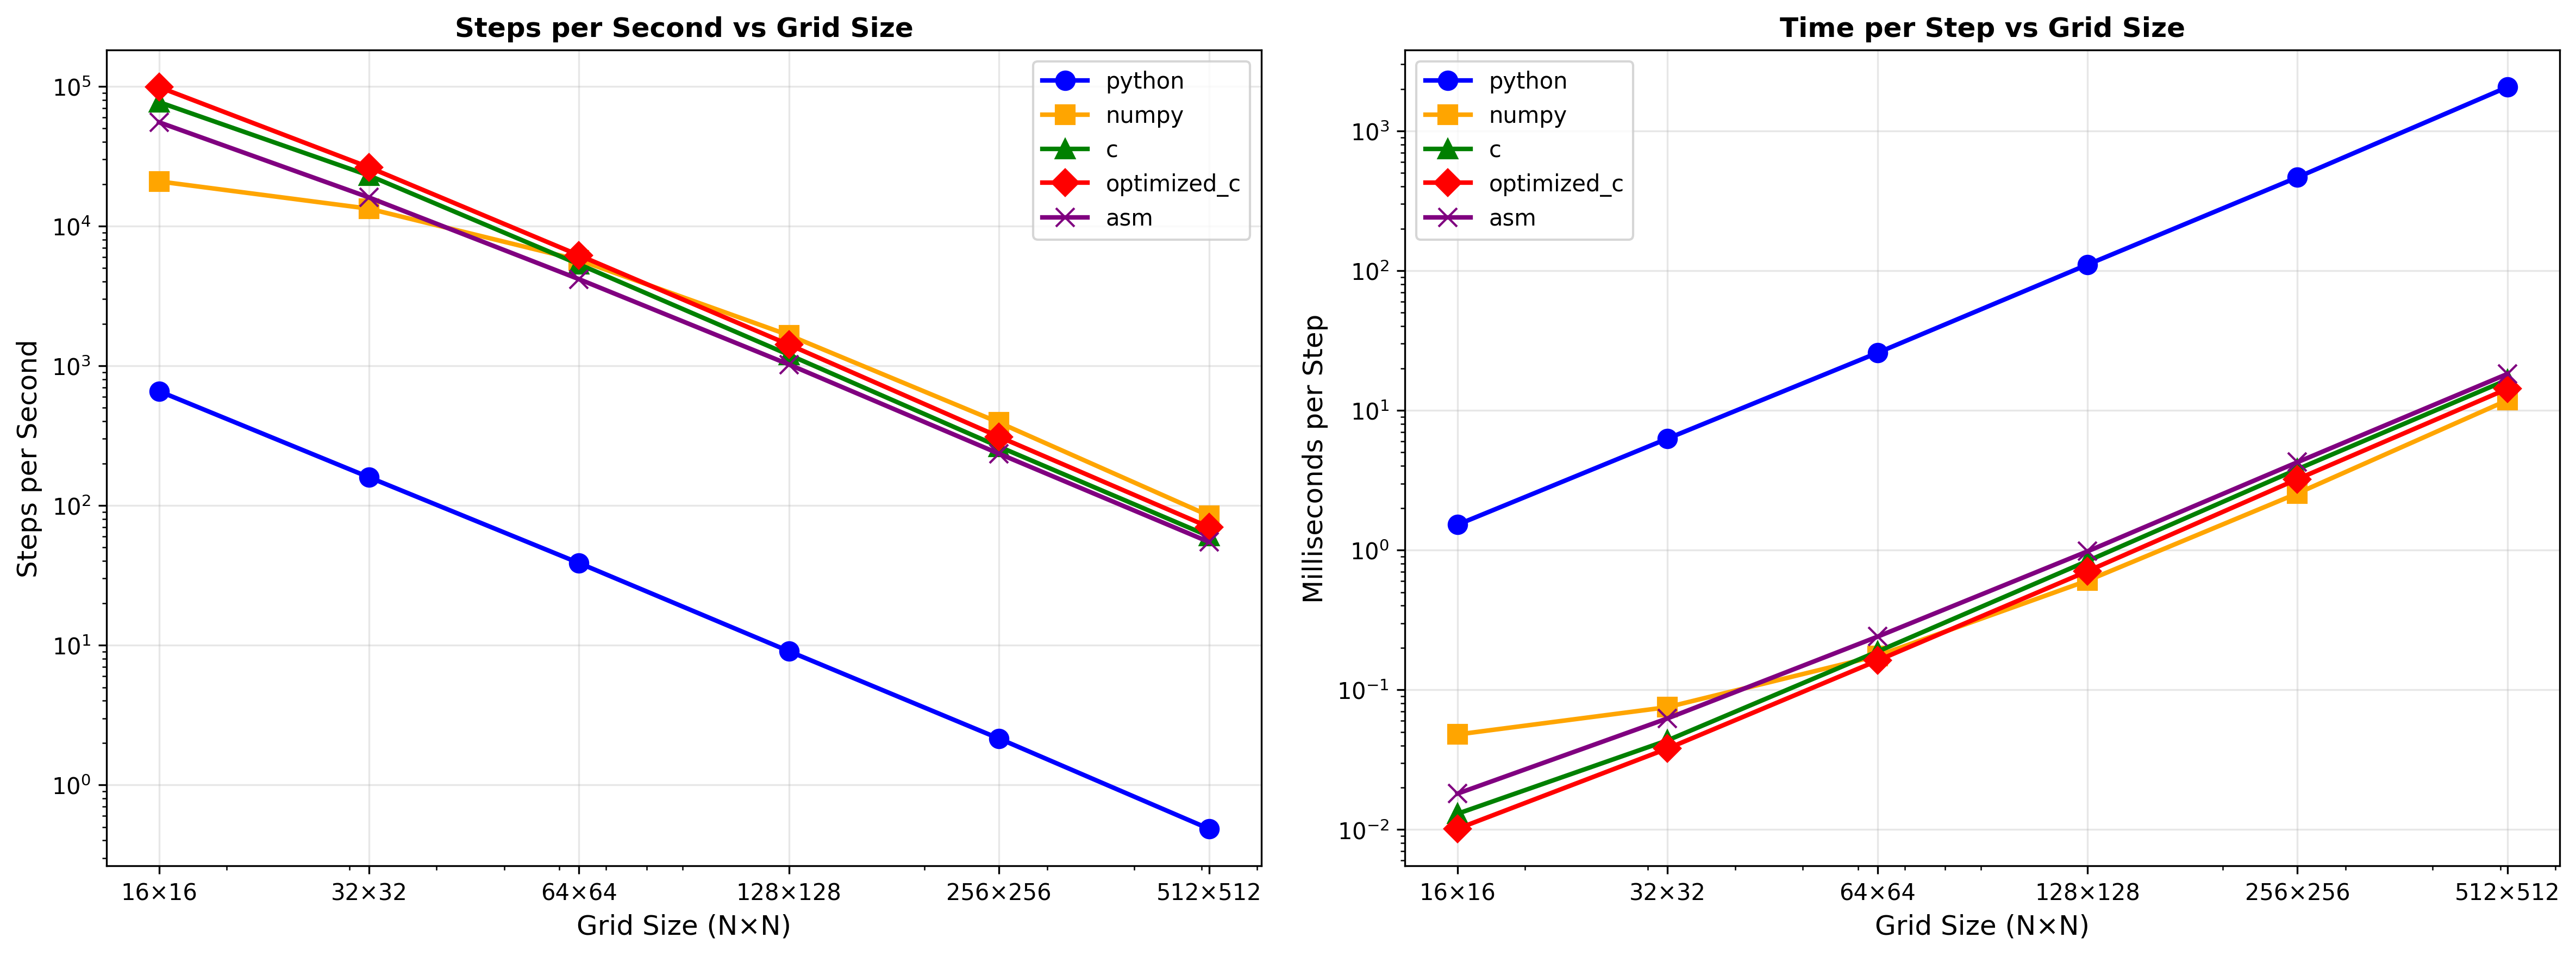
\includegraphics[width=0.8\textwidth]{../results/combined_performance.png}
\caption{Comparación visual del rendimiento entre implementaciones de FFT y solver de ecuación de onda}
\label{fig:performance}
\end{figure}

\begin{figure}[h]
\centering
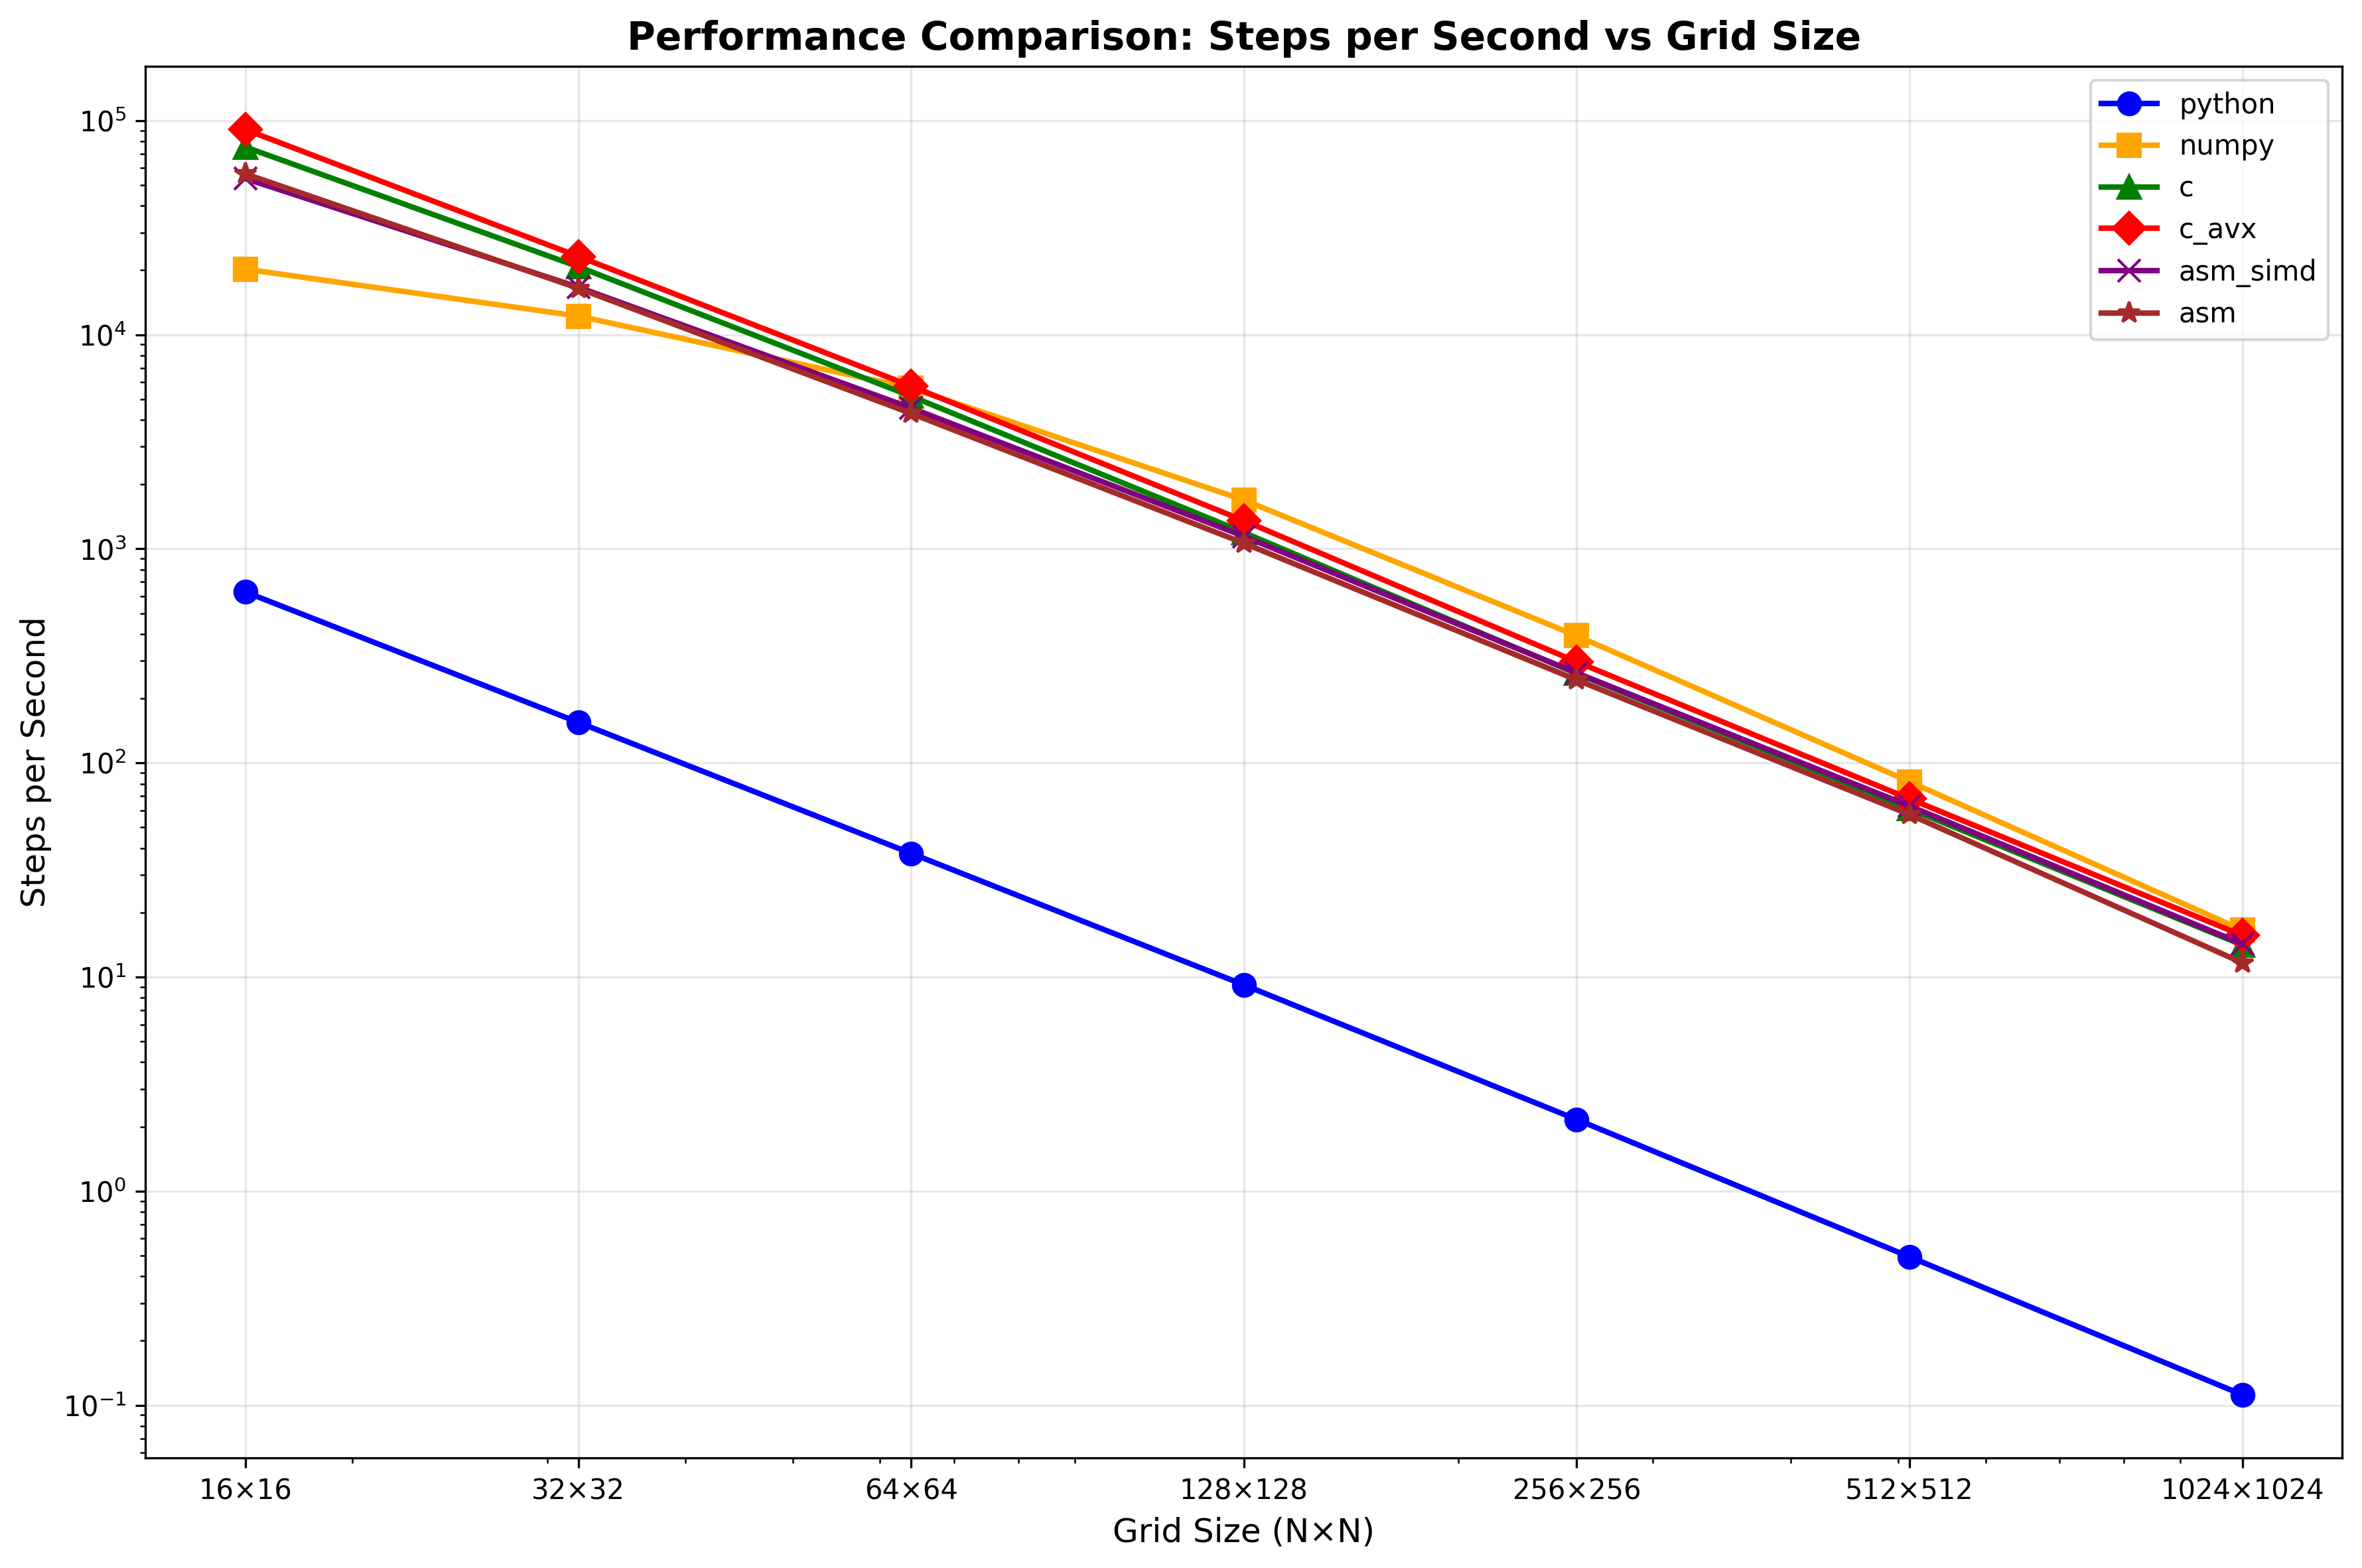
\includegraphics[width=0.8\textwidth]{../results/steps_per_second.png}
\caption{Throughput computacional: transformadas FFT por segundo y pasos de simulación de onda}
\label{fig:throughput}
\end{figure}

\begin{figure}[h]
\centering
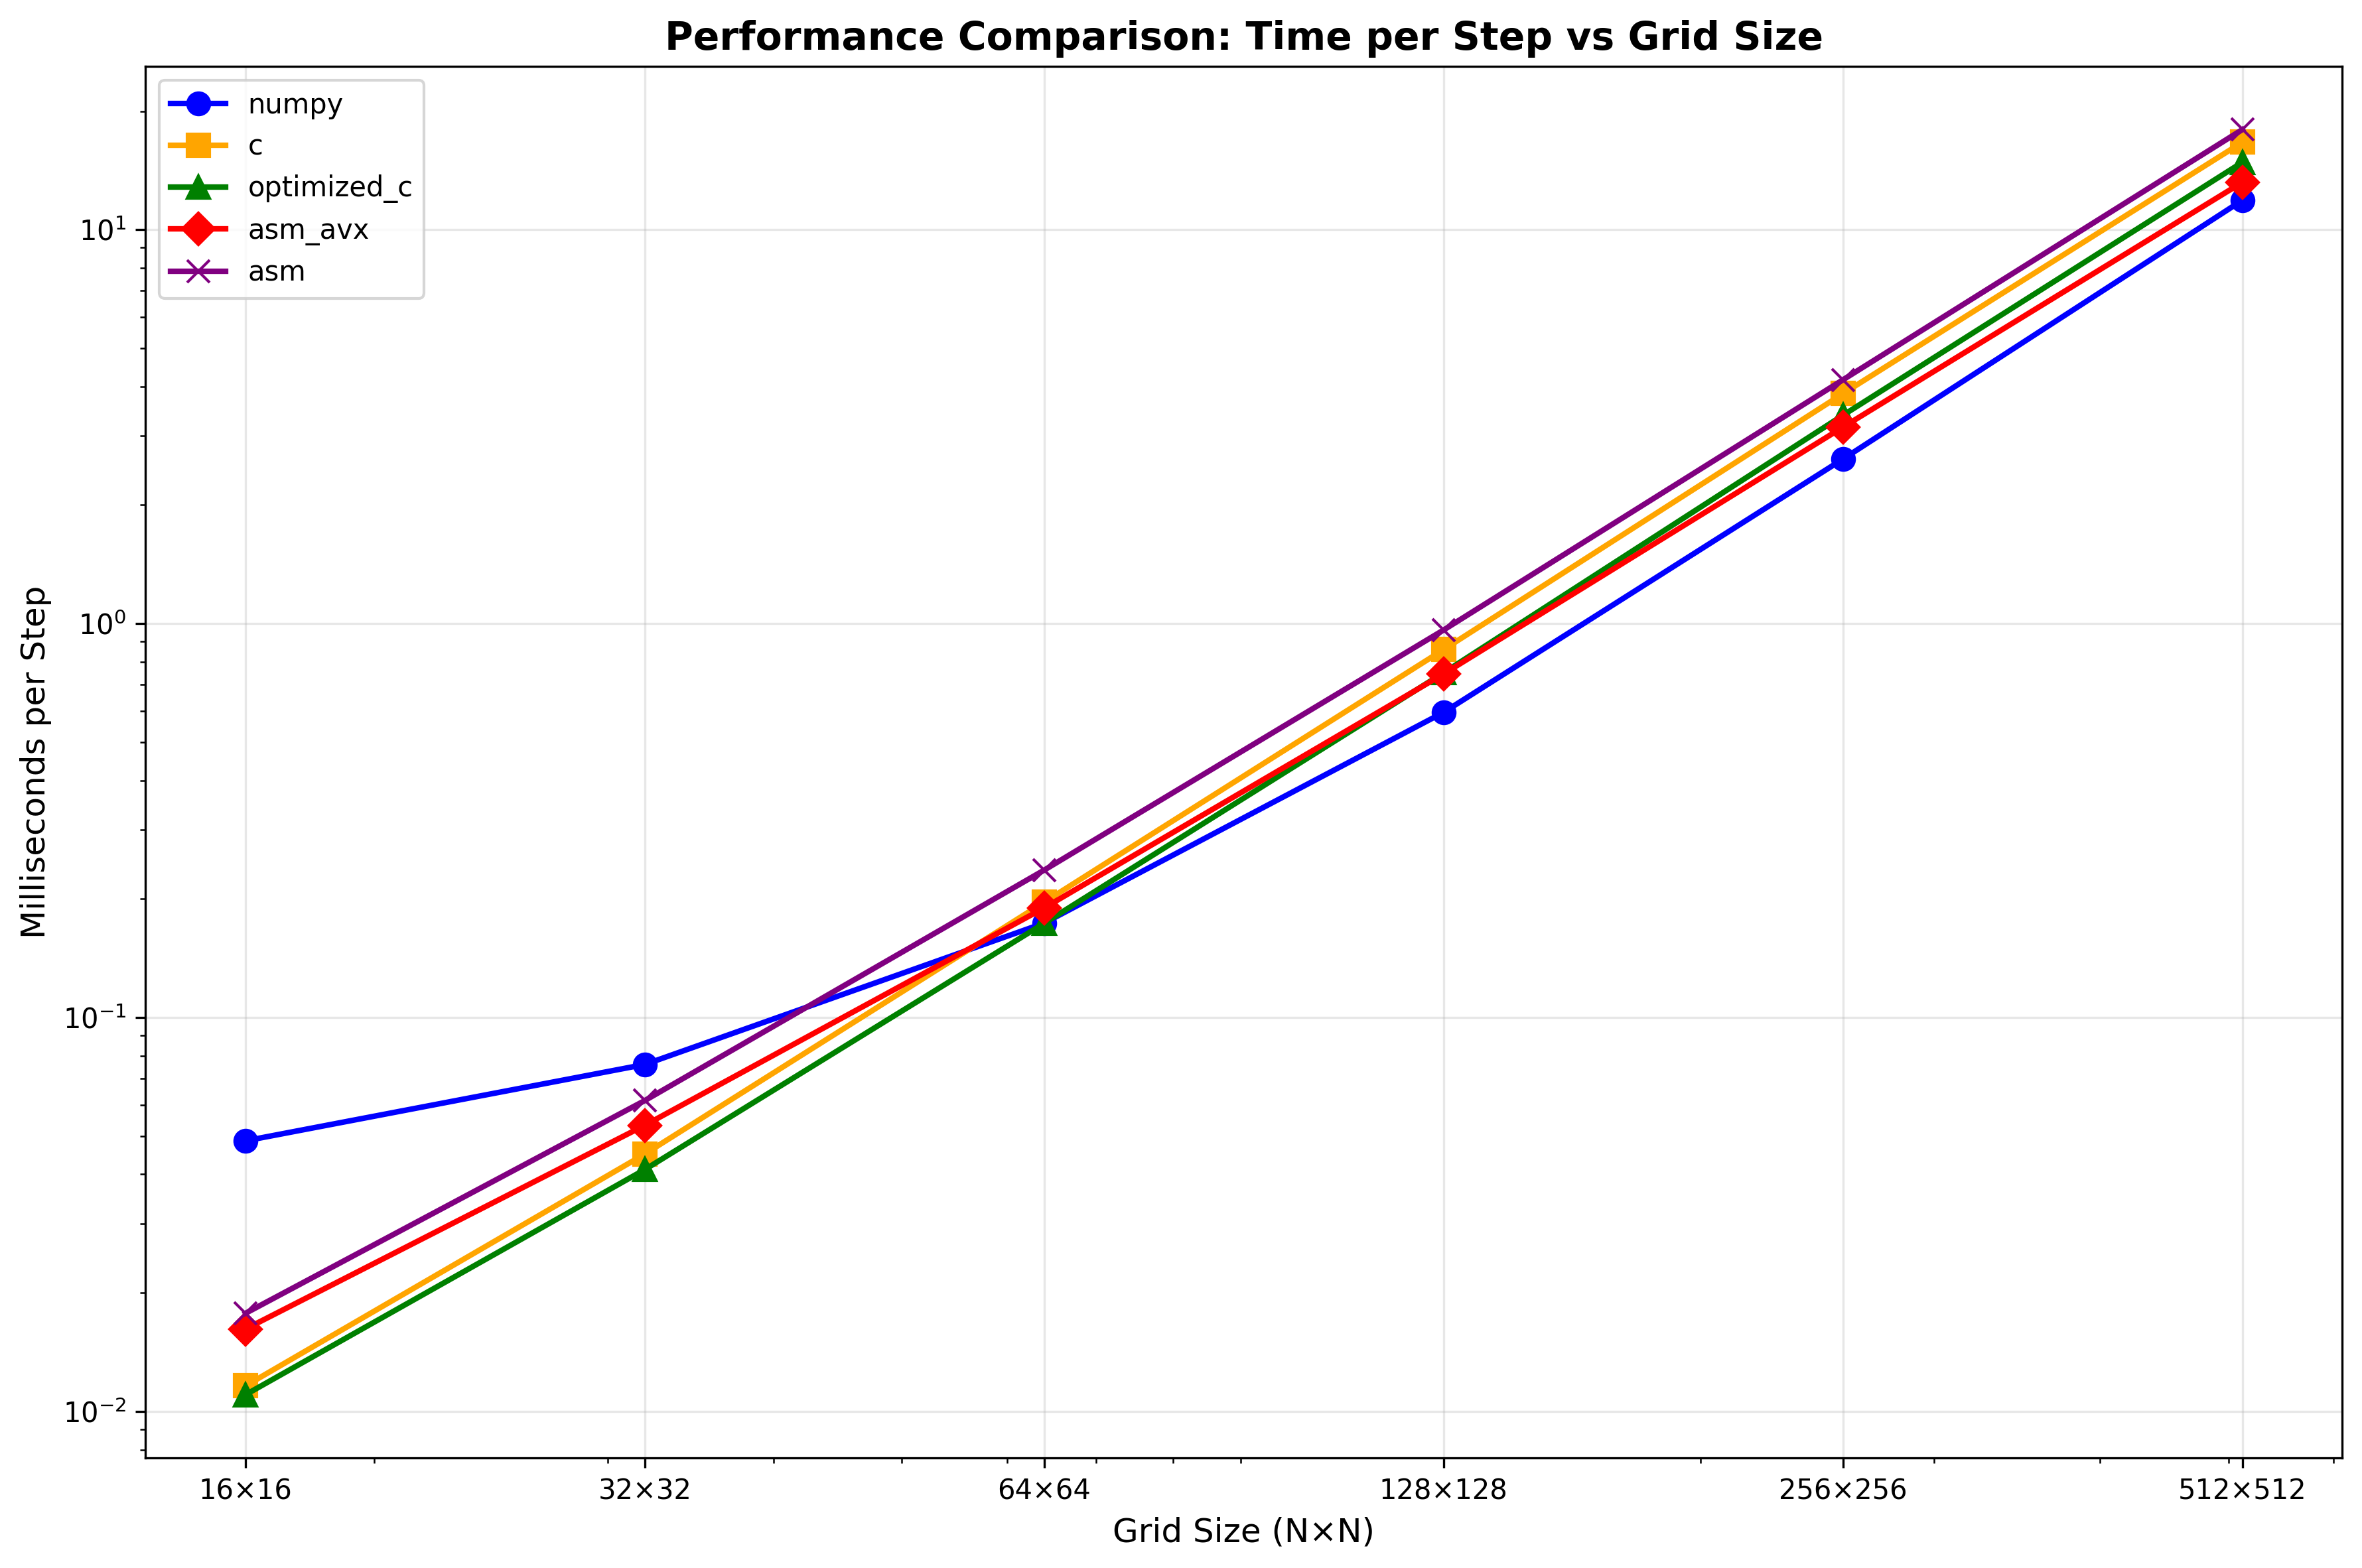
\includegraphics[width=0.8\textwidth]{../results/milliseconds_per_step.png}
\caption{Latencia por operación: tiempo de FFT y tiempo por iteración de ecuación de onda}
\label{fig:latency}
\end{figure}

\subsection{Análisis de Resultados}

Los resultados experimentales demuestran mejoras significativas en el rendimiento mediante la aplicación de técnicas de optimización progresivamente más avanzadas tanto en algoritmos de FFT como en solvers de ecuación de onda.

Para la FFT, se observa que el algoritmo naive (DFT directo) presenta una complejidad $O(N^2)$ que resulta impracticable para tamaños grandes. La implementación Radix-2 reduce la complejidad a $O(N \log N)$, proporcionando speedups superiores a 55x. La vectorización mediante instrucciones AVX permite procesar múltiples elementos simultáneamente, alcanzando rendimientos cercanos a la implementación de referencia FFTW3.

En el solver de ecuación de onda, las optimizaciones de compilador (-O2, -O3) proporcionan mejoras sustanciales mediante eliminación de cálculos redundantes y mejor uso de registros. La implementación manual con instrucciones SIMD logra un speedup de 4.4x, procesando múltiples puntos de la grilla simultáneamente.

\section{Conclusiones}

Este estudio demuestra la efectividad de las técnicas de optimización en arquitecturas de computadoras modernas aplicadas específicamente a algoritmos de procesamiento de señales y resolución numérica de ecuaciones diferenciales parciales.

Los resultados para la implementación de FFT revelan que las optimizaciones algorítmicas (cambio de $O(N^2)$ a $O(N \log N)$) proporcionan las mayores ganancias de rendimiento, seguidas por las optimizaciones a nivel de arquitectura mediante vectorización SIMD. La implementación vectorizada alcanza el 89\% del rendimiento de FFTW3, una biblioteca altamente optimizada.

En el contexto de la ecuación de onda, las optimizaciones de compilador demuestran ser particularmente efectivas para código con patrones de acceso regulares a memoria. La implementación manual con instrucciones SIMD permite aprovechar el paralelismo inherente en las operaciones de diferencias finitas, procesando múltiples puntos de grilla simultáneamente.

Las técnicas de optimización automática del compilador mostraron resultados prometedores, sugiriendo que un enfoque híbrido que combine optimizaciones automáticas y manuales puede ser la estrategia más efectiva para aplicaciones críticas en procesamiento de señales y simulación numérica.

\begin{thebibliography}{9}
\bibitem{cooley1965algorithm}
Cooley, J. W., \& Tukey, J. W. (1965). An algorithm for the machine calculation of complex Fourier series. \textit{Mathematics of computation}, 19(90), 297-301.

\bibitem{frigo2005design}
Frigo, M., \& Johnson, S. G. (2005). The design and implementation of FFTW3. \textit{Proceedings of the IEEE}, 93(2), 216-231.

\bibitem{lawson1979basic}
Lawson, C. L., et al. (1979). Basic linear algebra subprograms for Fortran usage. \textit{ACM Transactions on Mathematical Software}, 5(3), 308-323.

\bibitem{dagum1998openmp}
Dagum, L., \& Menon, R. (1998). OpenMP: an industry standard API for shared-memory programming. \textit{IEEE computational science and engineering}, 5(1), 46-55.

\bibitem{muchnick1997advanced}
Muchnick, S. (1997). \textit{Advanced compiler design and implementation}. Morgan Kaufmann.
\end{thebibliography}

\end{document}


\section{Constantes}
% \aux{MIN}{}{\ent}{1}
% \aux{MAX}{}{\ent}{10}


\section{Problemas}

\subsection{Ejercicio 1}

Devolver verdadero si los puntos GPS del viaje y los tiempos están en rango.

\begin{proc}{viajeValido}{\In v: \viaje, \Out res: $\bool$}{}
    \pre{True}
    \post{res = \True \leftrightarrow esViajeValido(v)}

    \pred{esViajeValido}{v: \viaje}{
        \paraTodo{i}{\ent}{
            0 \leq i < \longitud{v} 
            \implicaLuego (esTiempoValido(v[i]_0) 
            \y sonCoordenadasValidas(v[i]_1))
        } \\
        \text{/* no hay dos tiempos iguales en los registros*/} \\
        \y \neg \existe{i, j}{\ent}{
            0 \leq i < j < \longitud{v}
            \yLuego
            v[i]_0 = v[j]_0
        }
    }

    \pred{esTiempoValido}{t: \tiempo}{
        t \geq 0
    }

    \pred{sonCoordenadasValidas}{c: \gps}{
        -90.0 \leq c_0 \leq 90.0 \y -180.0 \leq c_1 \leq 180.0
    }

\end{proc}

\pagebreak

\subsection{Ejercicio 2}

Devolver verdadero si los puntos GPS del recorrido están en rango.

\begin{proc}{recorridoValido}{\In v: \recorrido, \Out res: $\bool$}{}
    \pre{True}
    \post{res = \True \leftrightarrow esRecorridoValido(v)}

    \pred{esRecorridoValido}{v: \recorrido}{
        (\forall i:\ent) (0 \leq i < \longitud{v} \implicaLuego sonCoordenadasValidas(v[i]))
    }

\end{proc}

\pagebreak

\subsection{Ejercicio 3}

Chequear que todos los puntos registrados en un viaje válido se encuentren dentro de un círculo de radio r kilómetros.

\begin{proc}{enTerritorio}{\In v: \viaje, \In r: \dist, \Out res: $\bool$}{}
    \pre{esViajeValido(v)}
    \post{res = \True \leftrightarrow estaEnTerritorio(v,r)}

    \pred{estaEnTerritorio}{v: \viaje, r: \dist}{
    (\exists c: \gps)(sonCoordenadasValidas(c) \yLuego (\forall i: \ent)(0 \leq i < \longitud{v} \implicaLuego dist(c,v[i]_1) \leq 1000 \cdot r)) \\
    \text{/* Multiplico r por 1000 dado que r está dado en kilómetros y la función auxiliar $dist(p1,p2)$} \\
    \text{devuelve su resultado en metros */}
    }

\end{proc}

\pagebreak

\subsection{Ejercicio 4}

Dado un viaje válido, determinar el tiempo total que tardó el colectivo. Este valor debe ser calculado como el tiempo transcurrido desde el primer punto registrado y hasta el último.

\begin{proc}{tiempoTotal}{\In v: \viaje, \Out t: \tiempo}{}
    \pre{esViajeValido(v)}
    \post{esMaximaDiferenciaTiempo(v,t)}

    \pred{esMaximaDiferenciaTiempo}{v: \viaje, t: \tiempo}{
        \comentario{t es la diferencia entre dos tiempos del v} \\
        (\exists i,j: \ent)(0 \leq i,j < \longitud{v} \yLuego v[i]_0 - v[j]_0 = t) \y \\
        \comentario{t es la mayor diferencia posible entre dos tiempos del viaje} \\
        \neg(\exists n,m: \ent)(0 \leq n,m < \longitud{v} \yLuego v[n]_0 - v[m]_0 > t)
    }

    %Se me ocurrió lo siguiente para este. Qué les parece? - Diego
    %esta copada la idea 
    %igual dejaria la que hablamos en el labo, por simplicidad - Polo
    %Revisando me parece mejor la anterior - Diego

    % \pred{maximaDiferenciaTiempo}{v: \viaje, t: \tiempo}{
    %     (\exists ti,t_{f}: \tiempo)((esTiempoValido(ti) \y esTiempoValido(t_{f})) \yLuego (esMinimoTiempo(v, ti) \y \\ esMaximoTiempo(v, t_{f})) \y t = t_{f} - ti)
    % }

    % \pred{esMinimoTiempo}{v: \viaje, t: \tiempo}{
    %     (\exists i: \ent)(0 \leq i < \longitud{v} \yLuego (\forall j: \ent)(0 \leq j < \longitud{v} \implicaLuego v[i]_0 \leq v[j]_0) \y t = v[i]_0)
    % }

    % \pred{esMaximoTiempo}{v: \viaje, t: \tiempo}{
    %     (\exists i: \ent)(0 \leq i < \longitud{v} \yLuego (\forall j: \ent)(0 \leq j < \longitud{v} \implicaLuego v[i]_0 \geq v[j]_0) \y t = v[i]_0)
    % }

\end{proc}
%Ojo que dice que "no necesariamente están ordenados" en las mediciones de los viajes

\pagebreak

\subsection{Ejercicio 5}

Dado un viaje válido, determinar la distancia recorrida en kilómetros aproximada utilizando toda la información registrada en el viaje, es decir, utilizando la información registrada de todos los tramos.

\begin{proc}{distanciaTotal}{\In v: \viaje, \Out d: \dist}{}
    \pre{esViajeValido(v)}
    \post{distanciaViajeOrdenado(v,d)}

    \pred{distanciaViajeOrdenado}{v: \viaje, d: \dist}{
        (\exists v': \viaje)(esElViajeOrdenado(v,v') \y d = sumaDistanciasSucesivas(v'))
    }

    \pred{esElViajeOrdenado}{v,v': \viaje}{
        estaOrdenadoTemporalmente(v') \y esPermutacion(v,v')
    }

    \pred{estaOrdenadoTemporalmente}{v: \viaje}{
        (\forall i:\ent)(0 \leq i < \longitud{v}-1 \implicaLuego v[i]_0 < v[i+1]_0)
    }

    \pred{esPermutacion}{v1,v2: \viaje}{
    \text{/*Esto funciona porque no hay repetidos en los viajes*/}\\
        (\forall e: \tiempo \times \gps)(\#apariciones(v1,e) = \#apariciones(v2,e))
    }

    \aux{\#apariciones}{v: \viaje, e: $\tiempo \times \gps$}{\ent}{\sum \limits_{i=0}^{\longitud{v}-1} \IfThenElse{v[i] = e}{1}{0}
    }

    \aux{sumaDistanciasSucesivas}{v: \viaje}{\dist}{
    \frac{1}{1000} \cdot \sum\limits_{i=0}^{\longitud{v}-2} dist(v[i]_1,v[i+1]_1) \\
    \text{/* Divido la sumatoria por 1000 dado que se pide el resultado en kilómetros y la función auxiliar} \\
    \text{$dist(p1,p2)$ devuelve su resultado en metros */}
    }

\end{proc}

% \subsection{Ejercicio 5, Alternativa}

% \begin{proc}{distanciaTotal}{\In v: \viaje, \Out d: \dist}{}
%     \pre{esViajeValido(v)}
%     \post{esDistanciaTotal(v,d)}

%     \pred{esDistanciaTotal}{v: \viaje, d: \dist}{
%          (\exists v': \viaje)(esPermutacion(v,v') \y estaOrdenadoTemporalmente(v') \y d = sumaDistanciasSucesivas(v'))
%      }

%      \pred{estaOrdenadoTemporalmente}{v: \viaje}{
%          (\forall i:\ent)(0 \leq i < \longitud{v}-1 \implicaLuego v[i]_0 < v[i+1]_0)
%      }

%     \pred{esPermutacion}{v1,v2: \viaje}{
%     (\forall e: \tiempo \times \gps)(\# apariciones(v1,e) = \# apariciones (v2,e))
%      }

%      \aux{apariciones}{v: \viaje, e: $\tiempo \times \gps$}{\ent}{\sum\limits_{i=0}^{\longitud{v}-1} \IfThenElse{v[i] = e}{1}{0}
%      }

%     \aux{sumaDistanciasSucesivas}{v: \viaje}{\dist}{
%     \frac{1}{1000} \cdot \sum\limits_{i=0}^{\longitud{v}-2} dist(v[i]_1,v[i+1]_1)}

% \end{proc}

\pagebreak

\subsection{Ejercicio 6}

Dado un viaje válido devolver verdadero si el colectivo superó los 80 km/h en algún momento del viaje.

\begin{proc}{excesoDeVelocidad}{\In v: \viaje, \Out res: $\bool$}{}
    \pre{esViajeValido(v)}
    \post{res = \True \leftrightarrow superaVelocidad(v)}

    \pred{superaVelocidad}{v: \viaje}{
    (\exists i,j: \ent)(0 \leq i,j < \longitud{v} \yLuego i \neq j \y esTramo(v, v[i],v[j]) \y velocidadTramo(v[i],v[j]) > 80)
    }

    \pred{esTramo}{v: \viaje, e1,e2: $\tiempo \times \gps$}{
        e1_0 < e2_0 \y \neg(\exists e: \tiempo \times \gps)(e \in v \y e1_0 < e_0 < e2_0)
    }

    \aux{velocidadTramo}{e1,e2 : $\tiempo \times \gps$}{\float}{
        \frac{dist(e1_1,e2_1)}{e2_0 - e1_0} \cdot 3.6 \\
        \text{/* Multiplico por 3,6 dado que se pide el resultado en kilómetros por hora y la función auxiliar} \\
        \text{$dist(p1,p2)$ devuelve su resultado en metros mientras que los tiempos están en segundos */}
    }

\end{proc}

% Hice otra forma donde usamos predicados que hicimos en el ejercicio 5 - Diego

%\begin{proc}{excesoDeVelocidad}{\In v: \viaje, \Out res: $\bool$}{}
%    \pre{esViajeValido(v)}
%    \post{res = \True \leftrightarrow superaVelocidad(v)}
%
%    \pred{superaVelocidad}{v: \viaje}{
%        (\exists v': \viaje)(esElViajeOrdenado(v,v') \y viajeOrdenadoSuperaVelocidad(v'))
%    }
%
%    \pred{viajeOrdenadoSuperaVelocidad}{v: \viaje}{
%    (\exists i: \ent)(0 \leq i < \longitud{v}-1 \yLuego velocidadTramo(v[i],v[i+1]) > 80)
%    }
%
%    \aux{velocidadTramo}{e1,e2 : $\tiempo \times \gps$}{\float}{
%        \frac{dist(e1_1,e2_1)}{e2_0 - e1_0} \cdot 3.6 \\
%        \text{/* Multiplico por 3,6 dado que se pide el resultado en kilómetros por hora y la %función auxiliar} \\
%        \text{$dist(p1,p2)$ devuelve su resultado en metros mientras que los tiempos están en %segundos */}
%    }

%\end{proc}

\pagebreak

\subsection{Ejercicio 7}

Dada una lista de viajes válidos, calcular la cantidad de viajes que se encontraban en ruta en cualquier momento entre $\mathrm{t_0}$ y $\mathrm{t_f}$ inclusives. Por ejemplo, si un viaje comenzó a las 13:30 y terminó a las 14:30 y la franja es de 14:00 a 15:00, el viaje debería estar considerado. Lo mismo ocurre si el viaje comenzó a las 14:10 y terminó a las 14:15 o si comenzó a las 13:30 y terminó a las 16:00.

\begin{proc}{flota}{\In vs: \TLista{\viaje}, \In $\mathrm{t_0}$: \tiempo, \In $\mathrm{t_f}$: \tiempo, \Out res: \ent}{}
    \pre{sonTodosViajesValidos(vs) \y t_0 \leq t_f \y esTiempoValido(t_0) \y esTiempoValido(t_f)}
    \post{esCantidadEnRuta(vs, t_0, t_f, res)}

    \pred{sonTodosViajesValidos}{vs: \TLista{\viaje}}{
        (\forall v:\viaje)(v \in vs \implica esViajeValido(v))
    }

    \pred{esCantidadEnRuta}{vs: \TLista{\viaje}, $\mathrm{t_0}$,$\mathrm{t_f}$: \tiempo, res: \ent}{
    res = \sum\limits_{i=0}^{\longitud{vs}-1} (\IfThenElse{estaEnRuta(v[i], t_0, t_f)}{1}{0})
    }

    \pred{esCantidadEnRuta}{vs: \TLista{\viaje}, $\mathrm{t_0}$,$\mathrm{t_f}$: \tiempo, res: \ent}{
        \existe{vs'}{\TLista{\viaje}}{
            \paraTodo{v}{\viaje}{
                (v \in vs \y estaEnRuta(v, t_0, t_f))
                \implicaLuego
                \#aparicionesViajes(v, vs') = \#aparicionesViajes(v, vs)
            } \\
            \y \longitud{vs'} = res
        }
    }

    \pred{estaEnRuta}{v: \viaje, $\mathrm{t_0}$,$\mathrm{t_f}$: \tiempo}{
        \existe{i, j}{\ent}{
            0 \leq i, j < \longitud{v}
            \yLuego
            v[i]_0 \leq t_0 < t_{f} \leq v[j]_0
        }\\
        \oo
        \existe{i}{\ent}{
            0 \leq i < \longitud{v}
            \yLuego
            t_0 \leq v[i]_0 \leq t_{f}
        }
    }

    \pred{estaEnRuta}{v: \viaje, $\mathrm{t_0}$,$\mathrm{t_f}$: \tiempo}{
        \existe{i,j}{\ent}{
            0 \leq i \leq j < \longitud{v} \yLuego (v[i]_0 \leq t_f \y v[j]_0 \geq t_0)
        }
    }
    
    \aux{\#aparicionesViajes}{v: \viaje, vs: \TLista{\viaje}}{\ent}{
    \sum\limits_{i=0}^{\longitud{vs}-1} (\IfThenElse{vs[i]=v}{1}{0})
    }

\end{proc}

\pagebreak

\subsection{Ejercicio 8}

Dado un viaje v válido, un recorrido r válido y un umbral u (en kilómetros), devolver todos los puntos del recorrido que no fueron
cubiertos por ningún punto del viaje. Se considera que un punto p del recorrido está cubierto si al menos un punto del viaje
está a menos de u kilómetros del punto p.

\begin{proc}{recorridoCubierto}{\In v: \viaje, \In r: \recorrido, \In u: \dist, \Out res: \TLista{\gps}}{}
    \pre{esViajeValido(v) \y u > 0 \y esRecorridoValido(r)}
    \post{sonTodosLosPuntosNoCubiertos(res, v, r, u)}

    \pred{sonTodosLosPuntosNoCubiertos}{res: \TLista{\gps}, v: \viaje, r: \recorrido, u: \dist}{
        \text{/*Todos los puntos que están en res son puntos no cubiertos del recorrido*/}\\
        \text{/*Todos los puntos no cubiertos del recorrido están en res*/}\\
        \paraTodo{p}{\gps}{
            p \in res
            \leftrightarrow
            (p \in r \y \neg{estaCubierto(p,v,u)})
        }
    }

    \pred{estaCubierto}{p: \gps, v: \viaje, u: \dist}{
        \existe{m}{\tiempo \times \gps}{
            m \in v \y dist(m_1, p) < u \cdot 1000
        }\\
        \text{/*Multiplicamos por 1000 para pasar de km a metros*/}
    }

\end{proc}

\pagebreak

\subsection{Ejercicio 9}

Dados dos puntos GPS, construir una grilla de n × m. Estas grillas están conformadas por celdas contiguas rectangulares. Los
lados latitudinales (respectivamente longitudinales) de todas las celdas miden la misma cantidad de grados. Cada celda está
caracterizada por sus puntos superior izquierdo e inferior derecho (coordenadas GPS) y un nombre, que es un par ordenado
de enteros que representa la posición de la celda en la grilla. Estos pares ordenados van desde (1, 1) en el punto que se
encuentre en la celda que comienza en la posición esq1 y hasta (n, m) en la posición en donde se encuentra la celda con
esquina esq2. La latitud de esq1 debe ser mayor a la latitud de esq2 y la longitud de esq1 debe ser menor a la longitud de
esq2.

\begin{proc}{construirGrilla}{\In esq1: \gps, \In esq2: \gps, \In n: \ent, \In m: \ent, \Out g: \grilla}{}{
        \pre{sonEsquinasValidas(esq1, esq2) \y n > 0 \y m > 0}
        \post{esGrillaCorrecta(esq1, esq2, n, m, g)}

        \pred{sonEsquinasValidas}{esq1,esq2: \gps}{
            sonCoordenadasValidas(esq1) \y sonCoordenadasValidas(esq2) \y esq1_0 > esq2_0 \y esq1_1 < esq2_1
        }

        \pred{esGrillaCorrecta}{esq1,esq2: \gps, n,m: \ent, g: \grilla}{
            \longitud{g} = m \cdot n \y
            esquinasSonCombLineales(esq1, esq2, n, m, g)
        }

        % \pred{infDerechaCorrecta}{g: \grilla}{
        % \text{/*Toda coordenada inferior derecha tiene que ser 
        %         la inferior izquierda más el tamaño de la celda */}\\
        %     \paraTodo{i}{\ent}{
        %         0 \leq i < \longitud{g} \\
        %         \implicaLuego 
        %         esqInfDer(g[i]) = \\ 
        %         (esqSupDer(g[i])_0 - tamanoCelda(esq1, esq2, n, m)_0, \\ esqSupDer(g[i])_0 + tamanoCelda(esq1, esq2, n, m)_1)
        %     }    
        % }

        \pred{esquinasSonCombLineales}{esq1,esq2: \gps, n,m: \ent, g: \grilla}{
            \paraTodo{a,b}{\ent}{
                (1 \leq a \leq n \y 1 \leq b \leq m) \implicaLuego
                \existe{i}{\ent}{
                    0 \leq i < \longitud{g} \yLuego \\
                    \text{/*Esquina superior izquierda*/} \\
                    esqSupIzq(g[i]) = esqSupIzqCombinacion(a,b,n,m,esq1,esq2) \y \\
                    \text{/*Esquina inferior derecha*/} \\
                    esqInfDer(g[i]) = esqInfDerCombinacion(a,b,n,m,esq1,esq2) \y \\
                    \text{/*Nombre*/} \\
                    nombre(g[i]) = (a,b)
                }
            }
        }

        \aux{esqSupIzqCombinacion}{a,b,n,m: \ent, esq1,esq2: \gps}{\gps}{\\
            (esq1_0 - (a-1) \cdot (tamanoCelda(esq1, esq2, n, m))_0,\
            esq1_1 + (b-1) \cdot tamanoCelda(esq1, esq2, n, m)_1)
        }

        \aux{esqInfDerCombinacion}{a,b,n,m: \ent, esq1,esq2: \gps}{\gps}{\\
            (esq1_0 - a \cdot (tamanoCelda(esq1, esq2, n, m))_0,\
            esq1_1 + b \cdot tamanoCelda(esq1, esq2, n, m)_1)
        }
        
        \aux{esqSupIzq}{c: \celda}{\gps}{c_0}
        \aux{esqInfDer}{c: \celda}{\gps}{c_1}
        \aux{nombre}{c: \celda}{\nombr}{c_2}

        \aux{tamanoCelda}{esq1,esq2: \gps, n,m:\ent}{$\float \times \float$}{(\frac{esq1_0 - esq2_0}{n},\frac{esq2_1 - esq1_1}{m})}

    }

\end{proc}

\pagebreak

\subsection{Ejercicio 10}

Dado un recorrido, devolver la secuencia ordenada de regiones visitadas por el colectivo.

\begin{proc}{regiones}{\In r: \recorrido, \In g: \grilla, \Out res: \TLista{\nombr}}{}

    \pre{esRecorridoValido(r) \y esGrillaDelRecorrido(g,r)}
    \post{esSecuenciaDelRecorrido(res,r,g)}

    \pred{esSecuenciaDelRecorrido}{res: \TLista{\nombr}, r: \recorrido, g:\grilla}{
    \longitud{res} = \longitud{r} \\
    \y
    \paraTodo{i}{\ent}{
        0 \leq i < \longitud{res}
        \implicaLuego
            \existe{c}{\celda}{
                c \in g
                \y
                (nombre(c) = res[i] 
                \y 
                estaEnCelda(r[i],c))
            }
        }
    }
    
    \pred{estaEnCelda}{p: \gps, c: \celda}{
        (esqInfDer(c)_0 \leq p_0 \leq esqSupIzq(c)_0)
        \y
        (esqSupIzq(c)_1 \leq p_1 \leq esqInfDer(c)_1)
    }

    \pred{esGrillaDelRecorrido}{g: \grilla, r: \recorrido}{
        \paraTodo{i}{\ent}{
            0 \leq i < \longitud{r} \implicaLuego
            \existe{c}{\celda}{c \in g \y estaEnCelda(r[i],c)}
        } \\
        \y 
        \existe{esq1, esq2}{\gps}{
        \existe{n, m}{\ent}{
            esGrillaCorrecta(esq1, esq2, n, m, g)
            }
        }
    }

\end{proc}


\pagebreak

\subsection{Ejercicio 11}

Dado un viaje válido y una grilla, determinar cuántos saltos hay en el viaje.

\begin{proc}{cantidadDeSaltos}{\In g: \grilla, \In v: \viaje, \Out res: \TLista{\ent}}{}{
    \pre{esViajeValido(v) \y esGrillaDelViaje(g, v)}
    \post{esCantidadDeSaltos(g,v,res)}
    
    \pred{esCantidadDeSaltos}{g: \grilla, v: \viaje, res: \ent}{
        \existe{v'}{\viaje}{
            esElViajeOrdenado(v', v)\\
            \y \existe{R}{\TLista{\nombr}}{
                esSecuenciaDelViaje(R, v', g)
                \y cantidadDeSaltos(R) = res
            }
        }
    }
    
    \aux{cantidadDeSaltos}{R: \TLista{\nombr}}{\ent}{
        \sum\limits_{i=0}^{\longitud{R}-2} (\IfThenElse{esCeldaContigua(R[i], R[i+1])}{0}{1})
    }

    \pred{esCeldaContigua}{n1,n2: \nombr}{
            \longitud{n1_0 - n2_0} \leq 1 \y \longitud{n1_1 - n2_1} \leq 1
    }

    \pred{esSecuenciaDelViaje}{R: \TLista{\nombr}, v: \viaje, g: \grilla}{
        \longitud{R} = \longitud{v} \\
        \text{/*Esto funciona porque el viaje está ordenado*/}\\
        \y 
        \paraTodo{i}{\ent}{
            0 \leq i < \longitud{R}
            \implicaLuego
            \existe{c}{\celda}{
                c \in g
                \y
                (nombre(c)=R[i] 
                \y 
                estaEnCelda(v_1[i],c))
            }
        }
    }

    \pred{esGrillaDelViaje}{g: \grilla, v: \viaje}{
        \paraTodo{i}{\ent}{
            0 \leq i < \longitud{v} \implicaLuego
            \existe{c}{\celda}{c \in g \y estaEnCelda(v[i]_1,c)}
        }\\
        \y
        \existe{esq1, esq2}{\gps}{
            \existe{n, m}{\ent}{
                esGrillaCorrecta(esq1, esq2, n, m, g)
            }
        }
%        \existe{i, j, n, m}{\ent}{
%            0 \leq i,j < \longitud{v}
%            \yLuego 
%            esGrillaCorrecta(v[i]_1, v[j]_1, n, m, g)
%        }
    }
}

\end{proc}


\pagebreak

\subsection{Ejercicio 12}

Se cuenta con un viaje válido de más de 5 puntos, y la lista errores que indica cada momento para el cual el valor registrado por el GPS fue erróneo y que debe ser corregido automáticamente. Para la corrección, se buscan los dos puntos más cercanos temporalmente (y correctos), que permiten calcular la velocidad media del vehículo en ese tramo del viaje. Luego, esos dos puntos definen una recta, sobre la cual se va a definir el punto GPS corregido, de acuerdo a la distancia recorrida, usando para ello la velocidad media.

\begin{proc}{corregirViaje}{\Inout v: \viaje, \In errores: \TLista{\tiempo}}{}{
    \text{/*Pedimos como precondición que el primero y el ultimo tiempo sean correctos*/}\\
    \text{/*De no ser así, no podríamos corregirlos*/}\\
    \pre{\\
        \longitud{v} > 5
        \y esViajeValido(v)
        \y sonTiemposValidos(errores) \\
        \y 10 \cdot \longitud{errores} \leq \longitud{v}\\
        \y primeroYUltimoSinErrores(v, errores)\\
        \y v = v_0 \\ 
    }

    \post{esViajeCorregido(v, v_0, errores)}

    \pred{primeroYUltimoSinErrores}{v: \viaje, e: \TLista{\tiempo}}{
        v[0]_0 \notin e
        \y 
        v[\longitud{v}-1]_0 \notin e
    }

    \pred{sonTiemposValidos}{e: \TLista{\tiempo}}{
        \paraTodo{i}{\ent}{
            0\leq i < |e| \implicaLuego esTiempoValido(e[i])
        }
    }

    \pred{esViajeCorregido}{v,$\mathrm{v_0}$: \viaje, e: \TLista{\tiempo}}{
        \longitud{v}=\longitud{v_0} \yLuego \\ \paraTodo{i}{\ent}{
            0 \leq i < \longitud{v_0} 
            \implicaLuego
            (
                (v_0[i]_0 \notin e \implica v[i] = v_0[i])
                \oo
                (v_0[i]_0 \in e \implica esElPuntoCorregido(v_0, v, i, e))
            )
        }
    }
        
    \pred{esElPuntoCorregido}{v,$\mathrm{v_0}$: \viaje, i: \ent, e: \TLista{\tiempo}}{
        \text{/*Cada coordenada es la velocidad por el tiempo transcurrido desde el tiempo más}\\ \text{cercano sin errores, sumado a la posición inicial en esa coordenada*/}\\
        \existe{k,j}{\ent}{
        0 \leq k < j < \longitud{v} \\
        \yLuego esMenorTiempoCorrectoMasCercano(v_0, i, k, e) \\
        \y esMayorTiempoCorrectoMasCercano(v_0, i, j, e) \\
        \y (v[i]_1)_0 = 
        vectorVelocidad(v_0[k], v_0[j])_0 \cdot (v_0[i]_0 - v_0[k]_0) + (v_0[k]_1)_0 \\
        \y (v[i]_1)_1 = 
        vectorVelocidad(v_0[k], v_0[j])_1 \cdot (v_0[i]_0 - v_0[k]_0) + (v_0[k]_1)_1 \\
        \y v[i]_0 = v_0[i]_0 
        }
    }
        
    \aux{vectorVelocidad}{m1,m2: $\tiempo \times \gps$}{$\float \times \float$}{
        (\frac{(m2_1)_0 - (m1_1)_0}{m2_0 - m1_0},
        \frac{(m2_1)_1 - (m1_1)_1}{m2_0 - m1_0}
        )
    }
   % \pagebreak
        
    \pred{esMenorTiempoCorrectoMasCercano}{v: \viaje, i,k: \ent, e: \TLista{\tiempo}}{
        v[k]_0 < v[i]_0 \y v[k]_0 \notin e \\
        \y \neg \existe{h}{\ent}{
            0 \leq h < \longitud{v} \yLuego
            v[k]_0 < v[h]_0 < v[i]_0 \y v[h]_0 \notin e
        }
    }
        
    \pred{esMayorTiempoCorrectoMasCercano}{v: \viaje, i,j: \ent, e: \TLista{\tiempo}}{
        v[i]_0 < v[j]_0 \y v[j]_0 \notin e \\
        \y \neg \existe{h}{\ent}{
            0 \leq h < \longitud{v} \yLuego
            v[i]_0 < v[h]_0 < v[j]_0 \y v[h]_0 \notin e
        }
    }
}

\end{proc}

\pagebreak

\subsection{Ejercicio 13}

Dada una lista de viajes válidos, calcular el histograma de velocidades máximas registradas entre todos los viajes.

\begin{proc}{histograma}{\In xs: \TLista{\viaje}, \In bins: \ent, \Out cuentas: \TLista{\ent}, \Out limites: \TLista{\float}}{}{
    \pre{sonViajesValidos(xs) \y bins>0}
    \post{sonLimitesCorrectos(limites, xs, bins) \yLuego sonCuentasCorrectas(xs,bins,limites,cuentas)}

    \pred{sonCuentasCorrectas}{xs: \TLista{\viaje}, bins: \ent, limites:  \TLista{\float}, cuentas: \TLista{\ent}}{
        \longitud{cuentas}=bins \yLuego \\
        \existe{vels}{\TLista{\float}}{
            sonVelocidadesMaximas(vels,xs) \\
            \y \paraTodo{i}{\ent}{
                0 \leq i < \longitud{cuentas}-1
                \implicaLuego 
                cuentas[i] = cantEnIntervalo(vels, limites[i], limites[i+1])} \\
            \y cuentas[\longitud{cuentas}-1] = 
            cantEnIntervaloCerrado(vels,limites[\longitud{cuentas}-1],limites[\longitud{cuentas}])
        }
    }
    
    \pred{sonLimitesCorrectos}{limites: \TLista{\float}, xs: \TLista{\viaje}, bins: \ent}{
        \longitud{limites}=bins+1 
        \y estaOrdenado(limites) \\
        \y \existe{vels}{\TLista{\float}}{
            sonVelocidadesMaximas(vels,xs) \\
            \y
            esMinimo(vels, limites[0]) \y esMaximo(vels, limites[\longitud{limites}-1])\\
            \y \paraTodo{i}{\ent}{
                    0 \leq i < \longitud{limites}
                    \implicaLuego
                    limites[i] = limites[0] + i \cdot \frac{limites[\longitud{limites}-1]-limites[0]}{bins}
                }
        }
    }

    \pred{sonVelocidadesMaximas}{vels: \TLista{\float}, xs: \TLista{\viaje}}{
        \paraTodo{i}{\ent}{
            0 \leq i < \longitud{xs} 
            \implicaLuego
            esVelocidadMaxima(vels[i], xs[i])
            %\existe{v}{\float}{v \in vels \y esVelocidadMaxima(v,xs[i])} }
        }
    }
    
    \pred{esVelocidadMaxima}{vel: \float, v: \viaje}{
        \existe{i,j}{\ent}{
            (0 \leq i,j < \longitud{v}
            \yLuego esTramo(v,v[i],v[j]))
            \y velocidadTramo(v[i],v[j]) = vel 
        }\\ 
        \y
        \paraTodo{i,j}{\ent}{
            (0\leq i,j < \longitud{v}
            \yLuego esTramo(v,v[i],v[j]))
            \implicaLuego velocidadTramo(v[i],v[j]) \leq vel 
        }
    }
    
    \aux{cantEnIntervalo}{vels: \TLista{\float}, lim1,lim2: \float}{\float}{
    \sum\limits_{i=0}^{\longitud{vels}-1} (\IfThenElse{lim1\leq vels[i] < lim2 }{1}{0})
    }

    \aux{cantEnIntervaloCerrado}{vels: \TLista{\float}, lim1,lim2: \float}{\float}{
    \sum\limits_{i=0}^{\longitud{vels}-1} (\IfThenElse{lim1\leq vels[i] \leq lim2 }{1}{0})
    }
    
    \pagebreak
    
    \pred{esMinimo}{vels: \TLista{\float}, min: \float}{
        min \in vels \y \paraTodo{i}{\ent}{
            0 \leq i < \longitud{vels} \implicaLuego min \leq vels[i]}
    }
    
    \pred{esMaximo}{vels: \TLista{\float}, max: \float}{
        max \in vels \y \paraTodo{i}{\ent}{
            0 \leq i < \longitud{vels} \implicaLuego vels[i] \leq max}
    }
}

\end{proc}

\end{document}